\documentclass[conference]{IEEEtran}
\usepackage{lipsum}
\IEEEoverridecommandlockouts
\usepackage{cite}
\usepackage{amsmath,amssymb,amsfonts}
\usepackage{algorithmic}
\usepackage{graphicx}
\usepackage{textcomp}
\usepackage{hyperref}
\usepackage{xcolor}
\usepackage{listings}
\lstset{basicstyle=\ttfamily,
  showstringspaces=false,
  commentstyle=\color{red},
  keywordstyle=\color{blue}
}

\def\BibTeX{{\rm B\kern-.05em{\sc i\kern-.025em b}\kern-.08em
    T\kern-.1667em\lower.7ex\hbox{E}\kern-.125emX}}

\makeatletter
\newcommand{\linebreakand}{%
  \end{@IEEEauthorhalign}
  \hfill\mbox{}\par
  \mbox{}\hfill\begin{@IEEEauthorhalign}
}
\makeatother

\begin{document}

\title{Service meshes as a solution for developing technology-independent microservices
}

\author{

\IEEEauthorblockN{Dangendorf, Kilian}
\IEEEauthorblockA{\textit{ Angewandte Informatik (M. Sc.)} \\
\textit{Hochschule Hannover}\\
kilian.dangendorf@stud.hs-hannover.de}
\and
\IEEEauthorblockN{Kirch, Eike}
\IEEEauthorblockA{\textit{ Angewandte Informatik (M. Sc.)} \\
\textit{Hochschule Hannover}\\
eike.kirch@stud.hs-hannover.de}
\and
\IEEEauthorblockN{Rust, Christopher}
\IEEEauthorblockA{\textit{ Angewandte Informatik (M. Sc.)} \\
\textit{Hochschule Hannover}\\
christopher.rust@stud.hs-hannover.de}
\linebreakand 
\IEEEauthorblockN{Ottlik, Manuel}
\IEEEauthorblockA{\textit{ Angewandte Informatik (M. Sc.)} \\
\textit{Hochschule Hannover}\\
manuel.ottlik@stud.hs-hannover.de}
}

\maketitle
\thispagestyle{plain}
\pagestyle{plain}

\begin{abstract}
\lipsum[100]
\end{abstract}

% brauchen wir sowas?
\begin{IEEEkeywords}
service meshes, microservices, kubernetes, java, nodejs, scalability, high availability
\end{IEEEkeywords}

\section{Introduction}

A microservice is an autonomous service that maps a small task of a specific domain and provides message-based communication through a well-defined interface \cite[p. 18]{microservices-general}.

High autonomy, cohesion, and interoperability are among the quality characteristics of a microservice. High autonomy of microservices ensures that the application is independent, self-contained, and fail-safe. High cohesion is hoped to increase maintainability and fast localization of errors. Interoperability ensures speeding up integrations \cite[p. 208 ff.]{microservices-general}.

Powerful microservices frameworks such as Spring Boot or Spring Cloud represent common solutions for microservices development. Key goals such as high availability, scalability, and resilience are achieved by providing services such as circuit breaking, load balancing, and API gateways \cite{spring-cloud}. These services are provided by using a framework, which is usually bound to a single programming language.

However, this contradicts the technology independence approach \cite{from-monolith} to microservices. This paper aims to shed light on whether and how service meshes can provide a solution to this problem.

\section{challenges of microservices}

The essential characteristic of a microservice architecture is to develop an application as a set of small and independent services. These run within their own process and are developed and deployed independently. Figure \ref{fig:microservice} illustrates the granularity of the microservice layer, where the business logic is designed to be very atomic. Each microservice should ideally have its focus on business logic \cite[p. 7]{sm3}.

Because of the granularity, the need for interservice communication increases. The complexity of this communication is usually more challenging than the actual business logic implementation. Due to the increased inter-service communication, microservices tend to be more prone to failures. This results in the requirement that a failure of one or more of these services should not bring down the entire application. Therefore, a failure of a microservice should be handled in such a way that it has minimal impact on the business functionalities of the application \cite[p. 11 ff.]{sm3}.

\begin{figure}
    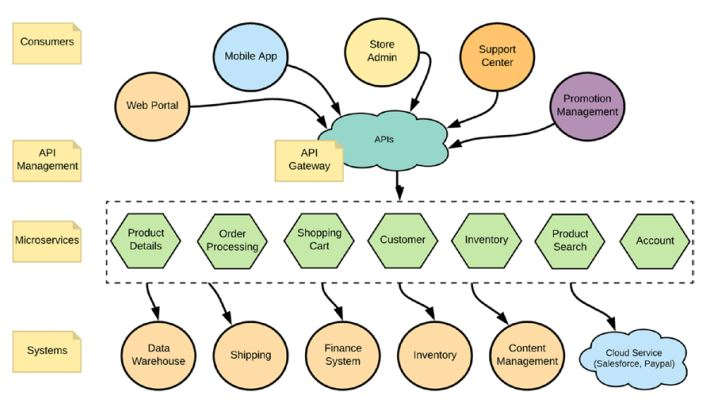
\includegraphics[width=\columnwidth]{img/microservice.JPG}
    \caption{Ex. microservice architecture of an online retail application \cite[p. 7]{sm3}}
    \label{fig:microservice}
\end{figure}

Another important challenge in the microservice context is maintenance. Due to the complexity of the architecture, it is necessary to introduce appropriate tools for e.g. service monitoring \cite[p. 16]{sm3}.
\section{Introduction to Docker and Kubernetes}

According to Google Trends, one of the most widespread solutions for microservices is \textsc{Kubernetes}.
To understand practical solutions of service meshes, it is very helpful to know how \textsc{Kubernetes} works. Since \textsc{Kubernetes} is often used together with \textsc{Docker}, this tool is also briefly explained.

\subsection{Docker}

\textsc{Docker} is a tool to encapsulate applications in so-called containers. It is built on Linux user groups and namespaces. Compared to a virtual machine, \textsc{Docker} is much more lightweight. All containers on the same host machine share the operating system kernel. Therefore, the overhead of booting the operating system for each container is eliminated \cite[p. 220 ff.]{sm3}.

Microservices are often deployed as so-called \textsc{Docker} images. This is a package consisting of the application and all its dependencies. The application itself only has access to the dependencies running in the image. The build process of a \textsc{Docker} image is defined in a so-called \textsc{Dockerfile} \cite[p. 224]{sm3}.

\subsection{Kubernetes}

\textsc{Kubernetes} provides a number of functions. It can be seen as a container platform, microservices platform and cloud platform.
It is a common way to use container technologies nowadays. Containers are isolated; they do not have access to processes or file systems of the host or other containers.
Advantages of container solutions are easy creation and deployment of container images that allow continuous integration, delivery and test. The role of \textsc{Kubernetes} is to manage and orchestrate these containers \cite{k8s}.

The four main \textsc{Kubernetes} objects are important to understand the role of service meshes in the microservices context:
\begin{itemize}
\item Pods: Pods are the smallest deployable unit that \textsc{Kubernetes} manages. A pod is one or a group of multiple containers that share storage and network resources.
\item Namespaces: Pods can be grouped into what are called namespaces. These represent a kind of virtual cluster. This already represents a kind of security concept. By default, a service from namespace A cannot communicate with a service from namespace B without explicit configuration.
\item Labels: Each \textsc{Kubernetes} deployment can be attached with an arbitrary amount of labels. These labels are simple key/value pairs that allow to group objects in \textsc{Kubernetes} into subsets \cite{k8s}.
\end{itemize}
\section{Characteristics of Service Meshes}

\begin{figure*}
    \centering
    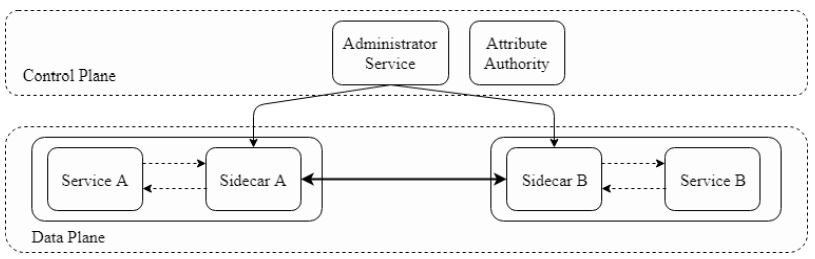
\includegraphics[width=0.8\textwidth]{img/mesh_detailed.JPG}
    \caption{Control and data plane in a service mesh\cite{sm4}}
    \label{fig:detailed mesh}
\end{figure*}


\begin{figure}
    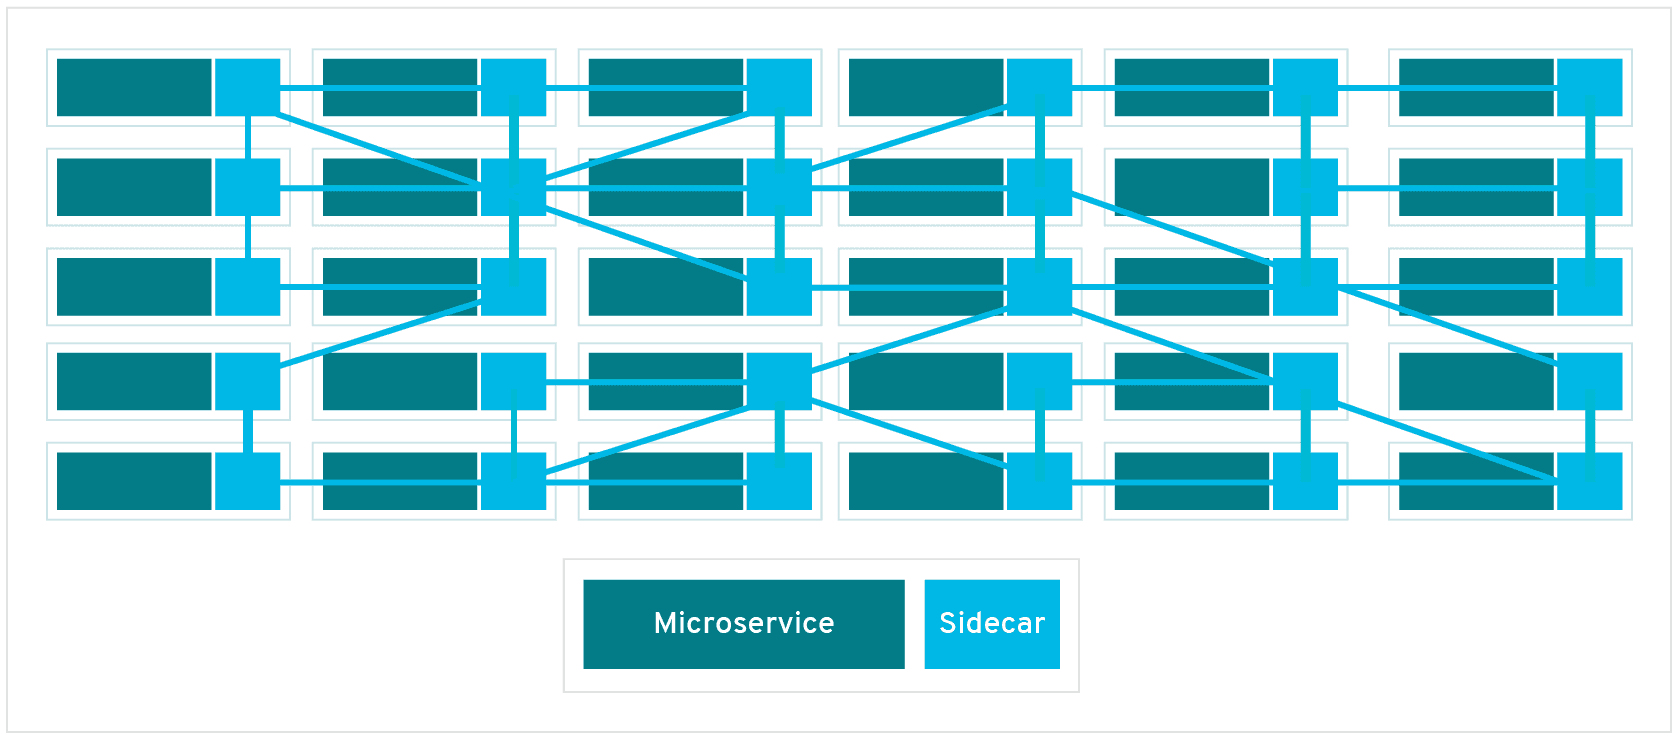
\includegraphics[width=\columnwidth]{img/mesh.png}
    \caption{Simplified service mesh based microservice architecture \cite{sm2}}
    \label{fig:overview}
\end{figure}

As mentioned in the previous chapter, creating an appropriate microservices infrastructure tend to be more complicated than implementing the business logic itself. For this reason, there is a need for infrastructure solutions that relieve the developers of the business logic. A service mesh is one conceivable solution approach and is defined as follows:

\subsection{Definition}

\begin{quote}
``A service mesh is a dedicated infrastructure layer for handling service-to-service communication. It’s responsible for the reliable delivery of requests through the complex topology of services that comprise a modern, cloud native application.
In practice, the service mesh is typically implemented as an array of lightweight network proxies that are deployed alongside application code, without the application needing to be aware." \cite[p. 123]{sm1}
\end{quote}

The last sentence of the definition sounds promising: The developer no longer has to worry about the infrastructure tasks. In the context of this paper, it should become clear how decoupled the infrastructure layer actually is.

\subsection{Architecture}
\label{chap:mesh-architecture}

Figure \ref{fig:overview} shows a simplified microservice architecture using service meshes. The mentioned infrastructure layer is a composition of the lightweight network proxies, also called sidecars. These sidecars control the entire network communication between the microservice instances. Without service mesh, each service must implement this interservice logic on its own, which compromises developer focus on business goals. The figure perfectly illustrates that application services are decoupled from interservice communication.

A more detailed illustration of a service mesh architecture is shown in figure \ref{fig:detailed mesh}. A service mesh consists of a control plane and a data plane.
The control plane is responsible for administrative tasks. This is where, for example, system-wide authentication and authorization policies are configured and made available to the proxies. Furthermore, settings for circuit breaking, timeouts and load balancing are made here. The composition of all application services with their sidecar proxies is called data plane \cite{sm4}.

\subsection{Central tasks}

Each service mesh has specific tasks to solve to enable microservice operation. These are named and briefly introduced below \cite{sm1}:

\subsubsection{Service discovery}

The number of service instances and the states and configurations change more frequently. For this reason, middleware is required to serve as an intermediary. It would be very complicated if every service A had to know under which IP and which port it can reach service B.

\subsubsection{Load balancing}

A load balancer is necessary to skillfully distribute requests to a service among replicas when loads are higher.

\subsubsection{Fault tolerance}

The microservice application must not be overly dependent on individual replicas being in a faulty state. For this reason, the service mesh must solve the task of forwarding requests only to services that have a sufficient health state.

\subsubsection{Traffic monitoring}

All communication between all microservices must be recorded and made visible, for example, via a central dashboard. In addition to logging, it makes sense to display metrics and statistics for the individual services.

\subsubsection{Circuit breaking}
Microservices need to be resilient. One way to do this is to implement the circuit breaker pattern. If recurring connection errors are detected for a resource, access to this resource is blocked by the circuit breaker so that it is not overloaded further.

\subsubsection{Authentication and access control}

With the use of a service mesh, it should be easy to apply and remove certain policies for authentication and authorization. One such policy could be that access to Service A, which provides the database logic, is only allowed by Service B and no one else.

\subsection{Opportunities and risks}

\begin{figure}
    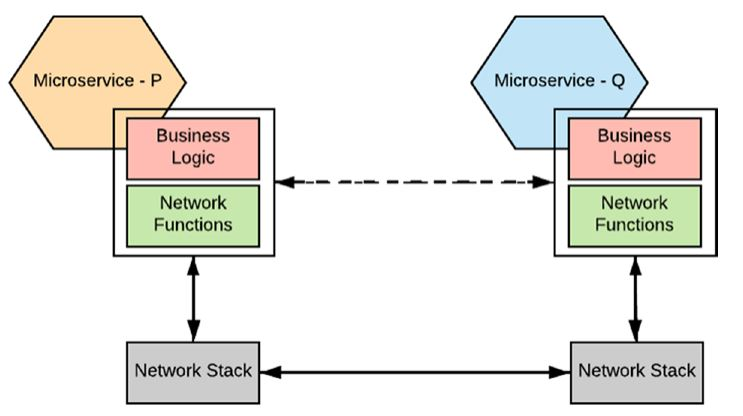
\includegraphics[width=\columnwidth]{img/microservices_without_mesh.JPG}
    \caption{Ex. architecture of microservices without service mesh\cite[S. 265]{sm4}}
    \label{fig:microservice-without-mesh}
\end{figure}


To highlight the benefits of a services mesh, you need to imagine a microservice architecture without services meshes. Figure 4 illustrates that each microservice requires a significant amount of logic to enable interservice communication. The effort required to implement this logic multiplies if, for example, Circuit Breaker is required in Java, Node.js, and Python. Since the requirements for infrastructure logic are the same in almost all microservice applications, it only makes sense to map this logic to an abstracted layer. This is where the service mesh comes into play. According to \cite{sm4}, the further advantages and drawbacks of a service mesh are as follows:

\subsubsection{Advantages}

\begin{itemize}

    \item Developers can concentrate on implementing their business applications. The management of a service mesh is more the task of an administrator or DevOps engineer.

    \item Polyglot support is another key benefit of service meshes. Developers can use their favorite programming languages and frameworks.

    \item In addition, the monitoring of services works out of the box. Distributed tracing and metrics require no additional effort from the developer's perspective. Furthermore, the application is decentralized, but centrally maintainable through the control plane. 

\end{itemize}
\subsubsection{Drawbacks}

\begin{itemize}
    \item On the other hand, service meshes also have disadvantages. Of course, the complexity of the architecture increases significantly by adding a sidecar proxy to each service instance. This also leads to the fact that each service call requires an additional hop.
    \item In addition, there are some problems in inter-service communication that service meshes do not address. These include complex routing, type mapping, and integration of other services and systems.
    \item A final important point is that service meshes are a comparatively new technology. The solutions are not necessarily mature enough for highly scaling environments.
\end{itemize}








\section{Solutions on the market}

The following chapter presents the two most popular solutions used in the context of service meshes: \textsc{Istio} and \textsc{Linkerd}. Both technology solutions have in common that they are based on \textsc{Kubernetes}. While \textsc{Linkerd} requires \textsc{Kubernetes}, \textsc{Istio} could also rely on virtual machines. To understand practical solutions of service meshes, it is very helpful to know how \textsc{Kubernetes} works. Since \textsc{Kubernetes} is often used together with \textsc{Docker}, this tool is also briefly explained.

\subsection{Docker}

\textsc{Docker} is a tool to encapsulate applications in so-called containers. It is built on Linux user groups and namespaces. Compared to a virtual machine, \textsc{Docker} is much more lightweight. All containers on the same host machine share the operating system kernel. Therefore, the overhead of booting the operating system for each container is eliminated \cite[p. 220 ff.]{sm3}.

Microservices are often deployed as so-called \textsc{Docker} images. This is a package consisting of the application and all its dependencies. The application itself only has access to the dependencies running in the image. The build process of a \textsc{Docker} image is defined in a so-called \textsc{Dockerfile} \cite[p. 224]{sm3}.

\subsection{Kubernetes}

\textsc{Kubernetes} provides a number of functions. It can be seen as a container platform, microservices platform and cloud platform.
It is a common way to use container technologies nowadays. Containers are isolated; they do not have access to processes or file systems of the host or other containers.
Advantages of container solutions are easy creation and deployment of container images that allow continuous integration, delivery and test. The role of \textsc{Kubernetes} is to manage and orchestrate these containers \cite{k8s}.

The four main \textsc{Kubernetes} objects are important to understand the role of service meshes in the microservices context:
\begin{itemize}
\item Pods: Pods are the smallest deployable unit that \textsc{Kubernetes} manages. A pod is one or a group of multiple containers that share storage and network resources.
\item Namespaces: Pods can be grouped into what are called namespaces. These represent a kind of virtual cluster. This already represents a kind of security concept. By default, a service from namespace A cannot communicate with a service from namespace B without explicit configuration.
\item Labels: Each \textsc{Kubernetes} deployment can be attached with an arbitrary amount of labels. These labels are simple key/value pairs that allow to group objects in \textsc{Kubernetes} into subsets \cite{k8s}.
\end{itemize}

Service meshes that use \textsc{Kubernetes} extend the functionality by abstracting concepts like automatic sidecar injection. This would be also possible without service meshes, but significantly more complex and less automated.

\subsection{Istio}

As illustrated in figure \ref{fig:arch-istio}, \textsc{Istio} uses a basic control and data plane architecture, as explained in chapter \ref{chap:mesh-architecture}. For the data plane, it uses the sidecar pattern by using \textsc{Envoy} proxies. \textsc{Envoy} a high-performance proxy that already brings features like service discovery, load balancing, circuit breaking and many more \cite{istio-docs-arch}.

\textsc{Istiod} (Istio daemon) provides management for service discovery, configuration and certificates. It converts routing rules into \textsc{Envoy}'s configuration format and also directs the traffic to the sidecar proxies \cite{istio-docs-arch}.

\begin{figure}
    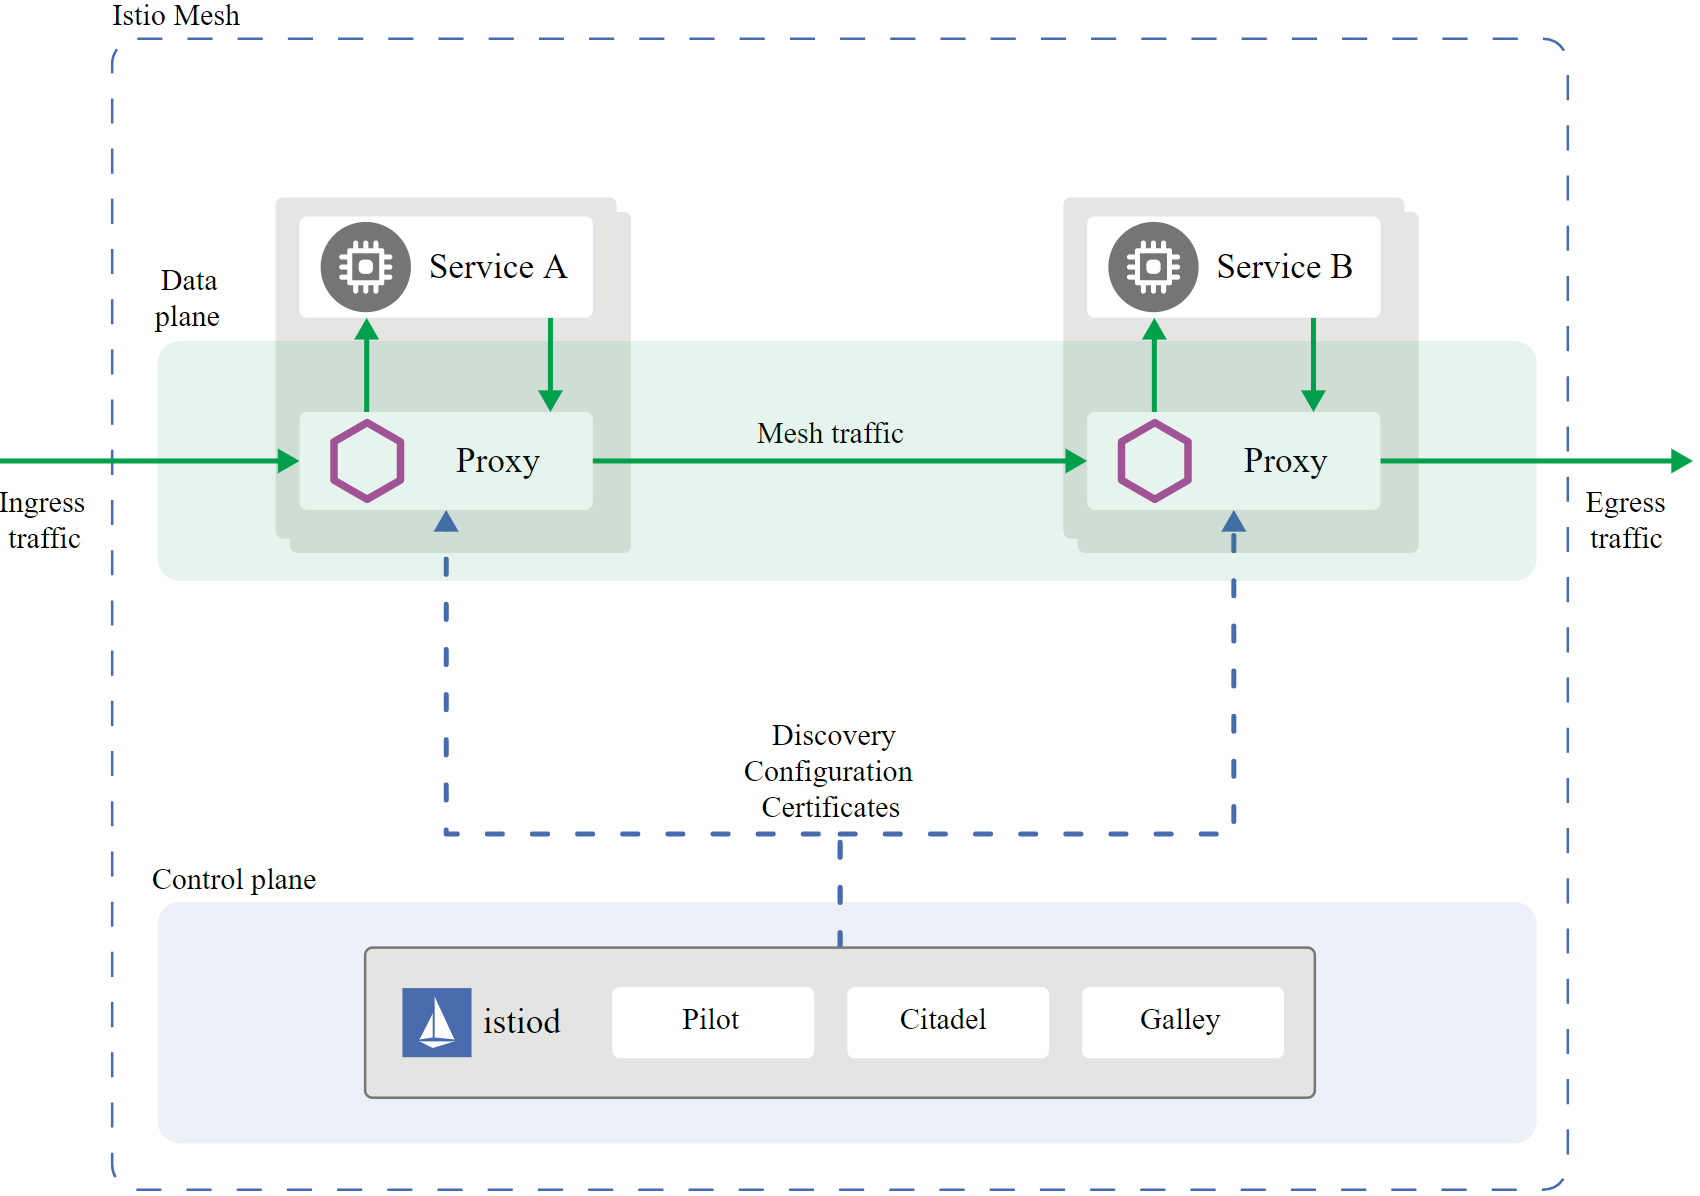
\includegraphics[width=\columnwidth]{img/istio_architecture.png}
    \caption{Architecture of \textsc{Istio} \cite{istio-docs-arch}}
    \label{fig:arch-istio}
\end{figure}

\subsection{Linkerd}
\label{linkerd}
According to \textsc{Linkerd}'s documentation \cite{linkerd-docs-arch}, \textsc{Linkerd} also uses a basic control and data plane architecture, as explained in chapter \ref{chap:mesh-architecture}. It also uses the sidecar pattern, but has implemented an own proxy solution named \textsc{Linkerd2-proxy}. \textsc{Linkerd} developers rate \textsc{Envoy} as too complex \cite{linkerd-docs-no-envoy}, which is why they decided to implement their own solution, which they call a "micro-proxy". 
Unlike \textsc{Istio}, \textsc{Linkerd} does not handle ingress traffic. It works in conjunction of every ingress controller of choice, e.g. \textsc{nginx} \cite{linkerd-docs-faq}.

As illustrated in figure \ref{fig:arch-linkerd}, each \textsc{linkerd-proxy} has access to two components: \textsc{identity} and \textsc{destination}.

\textsc{destination} is a lookup-service, where each proxy is able to check where exactly to send requests. \textsc{identity} provides a certificate authority.

While injecting a sidecar proxy on an application service, a route \textsc{/metrics} at port 4191 is exposed to provide log messages and metrics for \textsc{Prometheus}, which is a central logging and monitoring instance which is often used with \textsc{Kubernetes} \cite{linkerd-docs-arch}.

\begin{figure}
    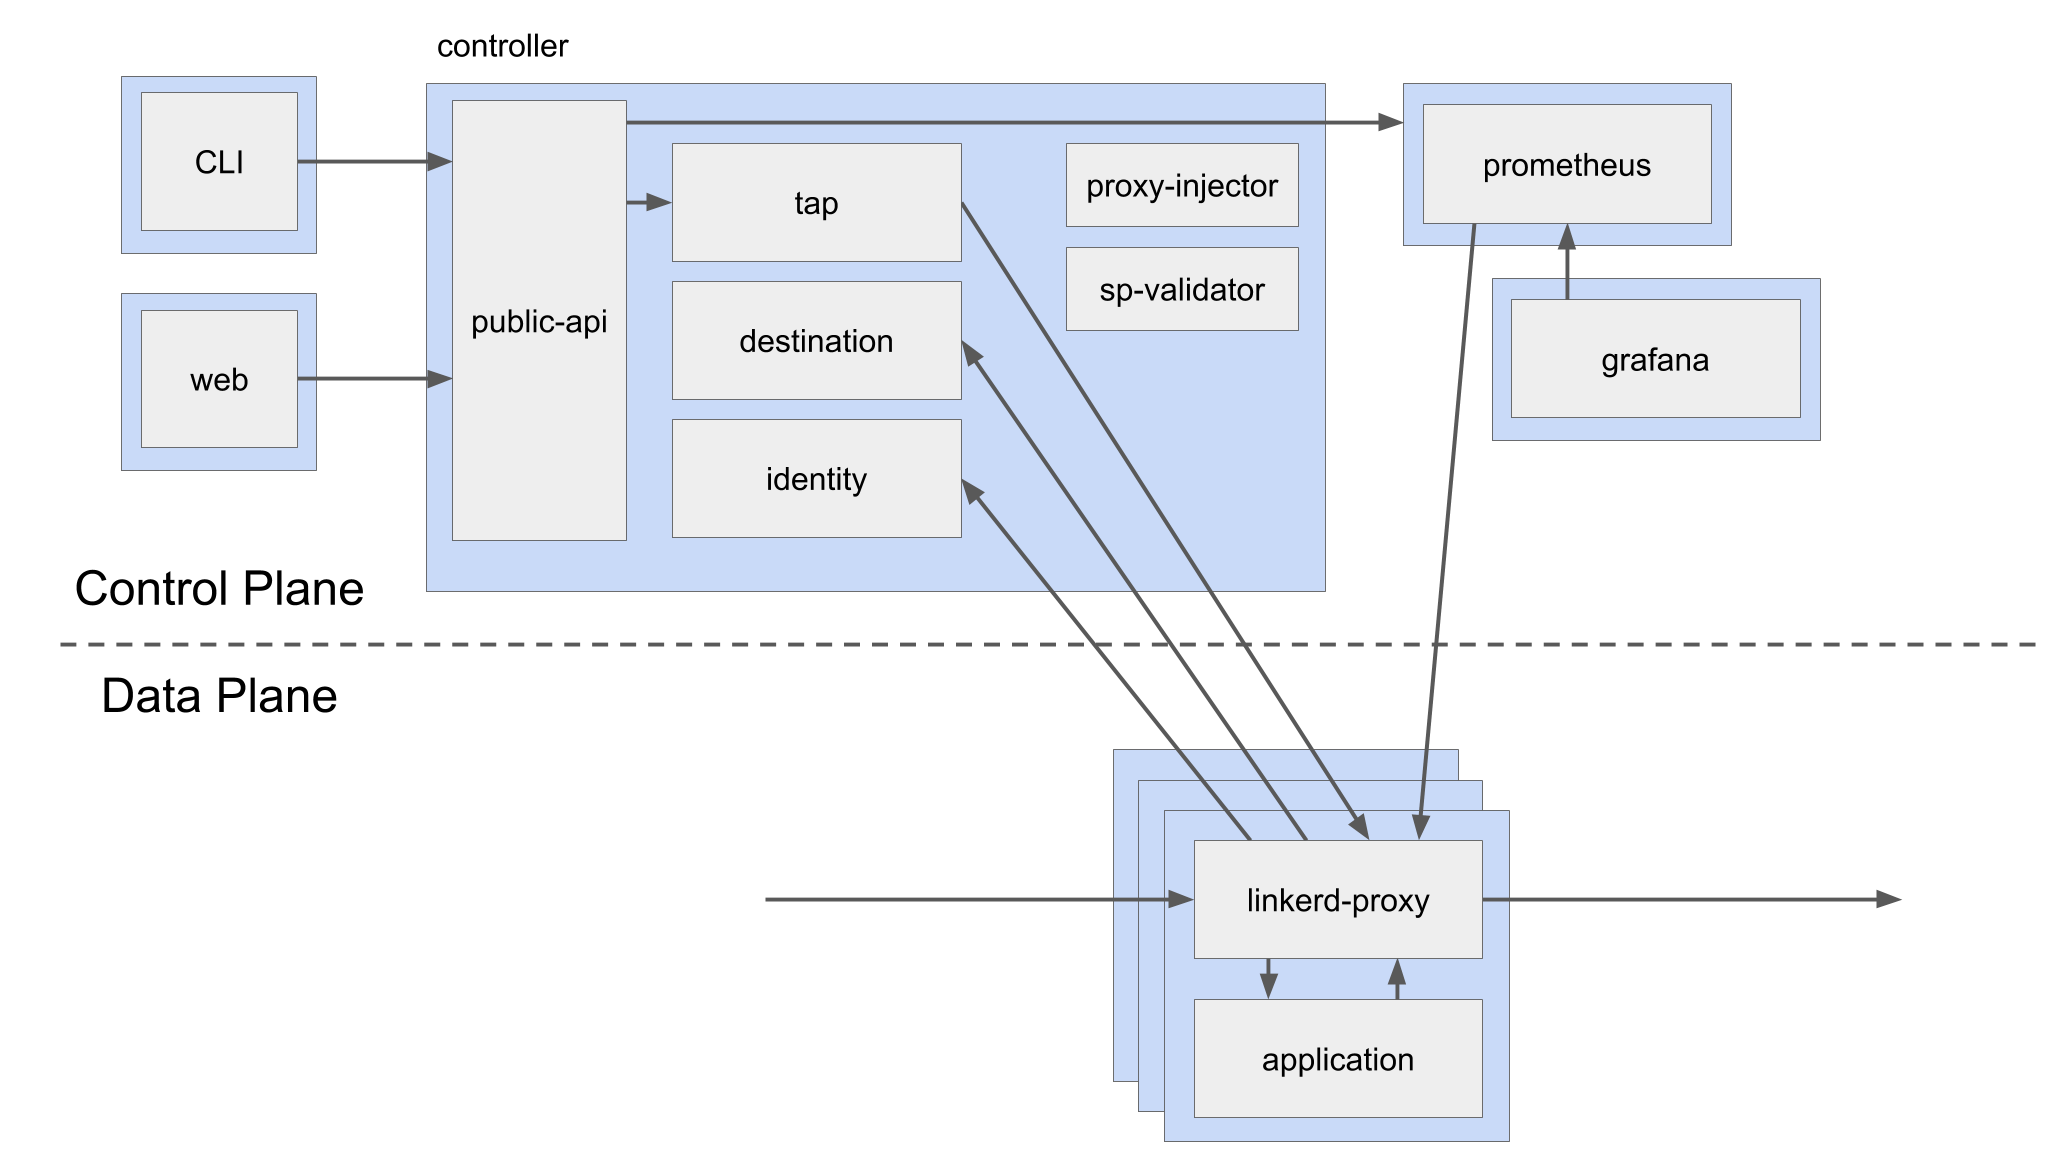
\includegraphics[width=\columnwidth]{img/linkerd_architecture.png}
    \caption{Architecture of \textsc{Linkerd} \cite{linkerd-docs-arch}}
    \label{fig:arch-linkerd}
\end{figure}

\subsection{Comparison}

As stated before, two very popular solutions for service meshes are \textsc{Linkerd} and \textsc{Istio}. Table \ref{tab:istio-linkerd} summarizes the key aspects of both tools, according to \cite{linkerd-github}, \cite{istio-github}, \cite{istio-linkerd-compare-1} and \cite{istio-linkerd-compare-2}:

\begin{table}
\centering

\begin{tabular*}{\columnwidth}{c|c|c}
                                 & Istio                                                                                                              & Linkerd     \\\hline
Initiators & \begin{tabular}[c]{@{}c@{}}Lyft, IBM,\\Google\end{tabular}                                                          	& \begin{tabular}[c]{@{}c@{}}Buoyant, Cloud Native\\Foundation\end{tabular}                                                           \\\hline
License                 & \multicolumn{2}{c}{Apache 2.0}                                                                                                          \\\hline
Runs on                          & \begin{tabular}[c]{@{}c@{}}Kubernetes,\\VMs\end{tabular}                                                           & Kubernetes  \\\hline
Sidecar proxy                    & \multicolumn{2}{c}{Yes}                                                                                                          \\\hline
Supports mTLS                    & \multicolumn{2}{c}{Yes}                                                                                                          \\\hline
Certificate management           & \multicolumn{2}{c}{Yes}                                                                                                          \\\hline
Authentication and authorization & \multicolumn{2}{c}{Yes}                                                                                                          \\\hline
Blue/Green deployment            & \multicolumn{2}{c}{Yes}                                                                                                          \\\hline
Circuit breaking                 & Yes                                                                                                                & No          \\\hline
Fault injection                  & \multicolumn{2}{c}{Yes}                                                                                                          \\\hline
Rate limiting                    & \multicolumn{2}{c}{Yes}                                                                                                          \\\hline
Monitoring                       & \multicolumn{2}{c}{Yes, with Prometheus}                                                                                         \\\hline
Complexity                       & High                                                                                                               & Low         \\\hline
Starts on GitHub \cite{linkerd-github} \cite{istio-github}              & 26.2k & 6.6k        \\\hline
Open issues on GitHub \cite{linkerd-github} \cite{istio-github}                 & 817                                                                                                                & 257         \\\hline
Documentation                    & ++                                                                                                                 & +          
\end{tabular*}
\vspace{0.25mm}
\caption{Comparison between Isto and \textsc{Linkerd}}
\label{tab:istio-linkerd}
\end{table}


%
%
% Mehr Erklärung zu Linkerd?
%
%

From an operators perspective, \textsc{Istio} and \textsc{Linkerd} look quite similar. After installing the service mesh, there are two main usage aspects: One the one hand, operators need to inject sidecar proxies in the pods of the microservice. On the other hand, they need to apply pluggable resources in YAML format, that could define policies like the usage of TLS.

By executing the command listed in \ref{lst:istio}, all deployments from namespaceA automatically get a sidecar proxy injected, while listing \ref{lst:linkerd} shows the injection command of a single deployment when using \textsc{Linkerd}.

\begin{lstlisting}[language=bash,caption={Injection of sidecards into deployments of a namespace in \textsc{Istio}},label={lst:istio}]
#!/bin/bash
kubectl label namespace default \
	istio-injection=enabled
\end{lstlisting}

\begin{lstlisting}[language=bash,caption={Injection of sidecards into a deployment in \textsc{Linkerd}}, label={lst:linkerd}]
#!/bin/bash
cat deployment.yml | linkerd inject - \
	| kubectl apply -f -
\end{lstlisting}

%
% TODO: WRITE STUFF
% 

In our prototypical implementation, we will use \textsc{Linkerd} as a service mesh technology. As table \ref{tab:istio-linkerd} clarifies, \textsc{Linkerd} seems to be less complex and more lightweight compared to \textsc{Istio}. One missing key feature of \textsc{Linkerd} is circuit breaking, which is requested by users and currently under development \cite{linkerd-circuit-breaker}. Nevertheless, \textsc{Istio} seems to be more powerful and mature, has more users and functionalities. Along with this, the pool of tutorials and documentation is also larger.
We will choose \textsc{Linkerd} because of its lightweight nature. The setup of \textsc{Linkerd}'s hello world example looks pretty straight forward and suitable and appropriate for a proof of concept.
\section{Prototypical service mesh implementation}

\begin{figure*}
    \centering
    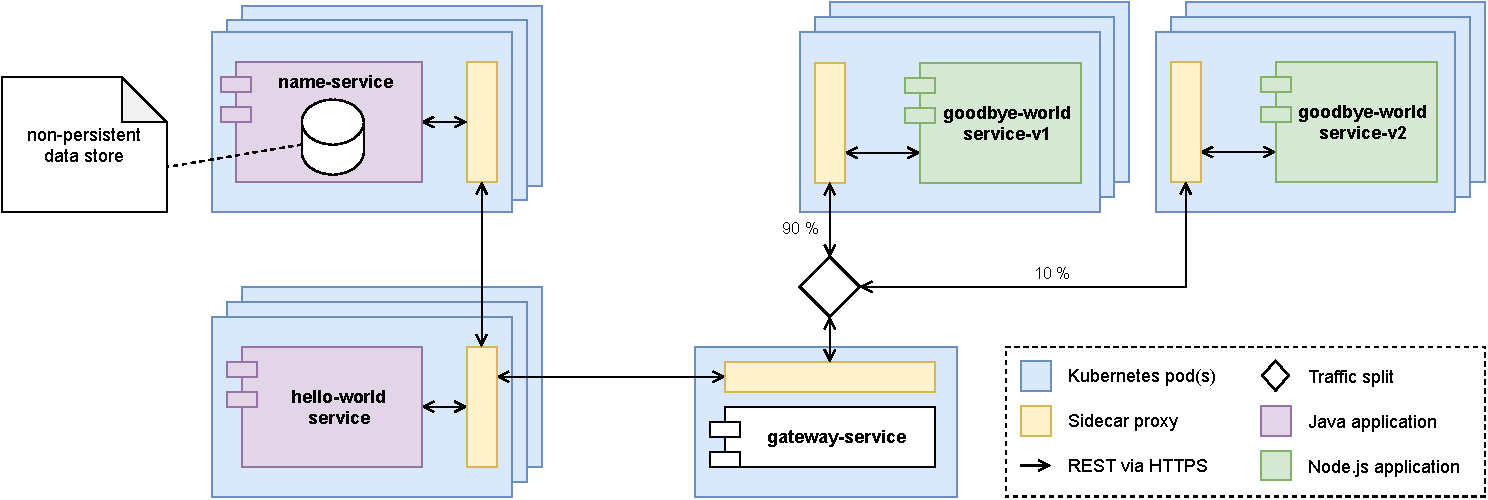
\includegraphics[width=\textwidth]{img/diagram-draft.pdf}
    \caption{Architecture overview of the PoC application}
    \label{fig:poc-overview}
\end{figure*}

\subsection{Choice of a mesh}

In our prototypical implementation, we used Linkerd as a service mesh technology. TODO: Justify why...

\subsection{Showcases}

\begin{itemize}
    \item Encryption
    \item Canary deployment
    \item Load balancing
    \item Central monitoring and logging
    \item Access policies
\end{itemize}
\section{Conclusion}

The theoretical and practical discussion of service meshes gave us very good impressions of the advantages and disadvantages of using them.
On the one hand, it is really very easy to apply or remove policies in the microservice architecture dynamically via customization of YAML resources. Powerful features such as circuit breaking, canary deployment, and centralized management ease the burden on both developers and operators of microservices architectures.

The proof of concept we presented using \textsc{Linkerd} hinted at the strengths and weaknesses of service meshes. It would certainly be interesting to take another look at Istio, as it promises a wider range of functions despite its higher complexity.

However, although \textsc{Linkerd} describes itself as lightweight, one aspect clearly emerged during the implementation of the proof of concept: The benefits of service meshes only come into play once the overall system is fully deployed. The creation of \textsc{Kubernetes} services and the commissioning of \textsc{Linkerd} require a high level of expert knowledge and effort. Consequently, it is rather utopian to integrate service meshes into a microservice landscape within a short time. However, once the first breakthrough has been achieved, the further development of new or existing microservices is comparatively more productive. The claim that developers can focus more on implementing the business logic is in line with our experience from dealing with \textsc{Linkerd}.
\begin{thebibliography}{00}

\bibitem{microservices-general} P. Giessler, ``Dom\"anengetriebener Entwurf von ressourcenorientierten Microservices'', Karlsruher Institut für Technologie (KIT), 2018

\bibitem{spring-cloud} 
Spring Cloud \url{https://spring.io/projects/spring-cloud} (Last access: 2021/02/11, 11 am)

\bibitem{from-monolith} R. Chen, S. Li and Z. Li, "From Monolith to Microservices: A Dataflow-Driven Approach," 2017 24th Asia-Pacific Software Engineering Conference (APSEC), Nanjing, 2017, p. 473

\bibitem{sm1} W. Li, Y. Lemieux, J. Gao, Z. Zhao and Y. Han, "Service Mesh: Challenges, State of the Art, and Future Research Opportunities," 2019 IEEE International Conference on Service-Oriented System Engineering (SOSE), San Francisco East Bay, CA, USA, 2019, pp. 122-1225

\bibitem{sm2} Was ist ein Service Mesh? - \url{https://www.redhat.com/de/topics/microservices/what-is-a-service-mesh} (Last access: 2021/02/11, 12 am)

\bibitem{sm3} Indrasiri, Kasun., and Prabath. Siriwardena. ``Microservices for the Enterprise": Designing, Developing, and Deploying / by Kasun Indrasiri, Prabath Siriwardena. 1st ed. 2018., Apress, 2018

\bibitem{sm4}
K. Y. Ponomarev, ``Attribute-Based Access Control in Service Mesh," 2019 Dynamics of Systems, Mechanisms and Machines (Dynamics), Omsk, Russia, 2019, pp. 1-4

\bibitem{linkerd-github} linkerd/linkerd2 @ GitHub - \url{https://github.com/linkerd/linkerd2} (Last access: 2021/02/17, 11 am)

\bibitem{istio-github} istio/istio @ GitHub - \url{https://github.com/istio/istio} (Last access: 2021/02/17, 11 am)

\bibitem{istio-linkerd-compare-1} Kubernetes Service Mesh: A Comparison of Istio, Linkerd and Consul - \url{https://platform9.com/blog/kubernetes-service-mesh-a-comparison-of-istio-linkerd-and-consul/} (Last access: 2021/02/17, 11 am)

\bibitem{istio-linkerd-compare-2} Service Mesh: Einführung \& Vergleich von Istio und Linkerd - \url{https://www.predic8.de/service-mesh-microservices.htm}  (Last access: 2021/02/17, 11 am)

\bibitem{linkerd-circuit-breaker} Circuit breaker support? - \url{https://github.com/linkerd/linkerd2/issues/2846} (Last access: 2021/02/17, 2 pm)

\bibitem{fowler} Microservices - \url{https://martinfowler.com/articles/microservices.html}

\bibitem{k8s} Konzepte | Kubernetes - \url{https://kubernetes.io/de/docs/concepts/}

\end{thebibliography}

\end{document}
